\documentclass{article}

\usepackage{tikz}
\usetikzlibrary{shapes,arrows}
\usetikzlibrary{decorations.pathreplacing}
\usetikzlibrary{decorations.pathmorphing}
\usetikzlibrary{decorations.markings}



\begin{document}
Here we have some example TikZ drawings to use as examples and templates.


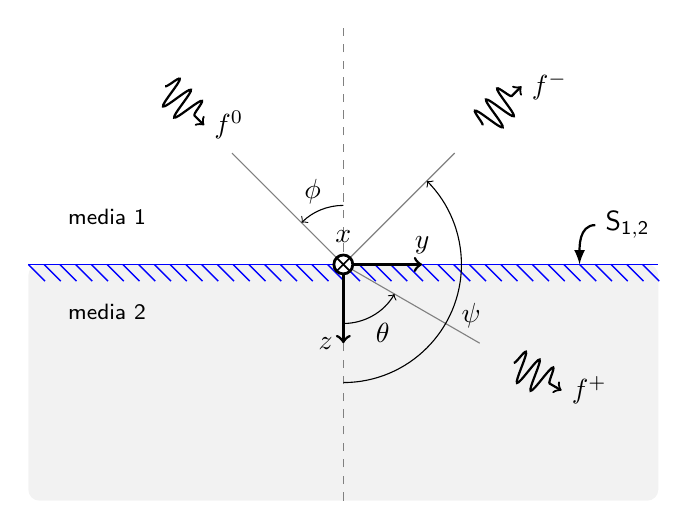
\begin{tikzpicture}[
    media/.style={font={\footnotesize\sffamily}},
    wave/.style={
        decorate,decoration={snake,post length=1.4mm,amplitude=2mm,
        segment length=2mm},thick},
    interface/.style={
        % The border decoration is a path replacing decorator. 
        % For the interface style we want to draw the original path.
        % The postaction option is therefore used to ensure that the
        % border decoration is drawn *after* the original path.
        postaction={draw,decorate,decoration={border,angle=-45,
                    amplitude=0.3cm,segment length=2mm}}},
    ]
    % Round rectangle
    \fill[gray!10,rounded corners] (-4,-3) rectangle (4,0);
    % Interface
    \draw[blue,line width=.5pt,interface](-4,0)--(4,0);
    % Vertical dashed line
    \draw[dashed,gray](0,-3)--(0,3);
    % Coordinates system
    \draw(0,0.15)node[above]{$x$};
    \draw[<->,line width=1pt] (1,0) node[above]{$y$}-|(0,-1) node[left]{$z$};
    % Incidence
    \draw[->,wave]
         (135:3.2cm)--(135:2.5cm)node[right]{$f^0$};
    \draw[gray](0:0cm)--(135:2cm);
    \path (0,0)++(113:1cm)node{$\phi$};
    \draw[->](0,0.75)arc(90:135:.75cm);
    % Transmission
    \draw[->,wave]
         (-30:2.5cm)--(-30:3.2cm)node[right]{$f^+$};
    \draw[gray](0:0cm)--(-30:2cm);
    \path (0,0)++(-60:1cm)node{$\theta$};
    \draw[->] (0,-0.75) arc (-90:-30:.75cm);
    % Reflection
    \draw[->,wave]
         (45:2.5cm)--(45:3.2cm)node[right]{$f^-$};
    \path (0,0)++(-22:1.75cm) node{$\psi$};
    \draw[gray](0:0cm)--(45:2cm);
    \draw[->] (0,-1.5)arc(-90:45:1.5cm);
    % Media names
    \path[media] (-3,.6)  node {media 1}
                 (-3,-.6) node {media 2};

    % $x$ axis
    \filldraw[fill=white,line width=1pt](0,0)circle(.12cm);
    \draw[line width=.6pt] (0,0)
                          +(-135:.12cm) -- +(45:.12cm)
                          +(-45:.12cm) -- +(135:.12cm);
    % Interface pointer
    \draw[-latex,thick](3.2,0.5)node[right]{$\mathsf{S_{1,2}}$}
         to[out=180,in=90] (3,0);
    % To-paths are really useful for drawing curved lines. The above
    % to path is equal to:
    %
    % \draw[-latex,thick](3.2,0.5)node[right]{$\mathsf{S_{1,2}}$}
    %      ..controls +(180:.2cm) and +(up:0.25cm) .. (3,0);
    % Internally the to path is translated to a similar bezier curve,
    % but the to path syntax hides the complexity from the user. 
\end{tikzpicture}

\begin{center}
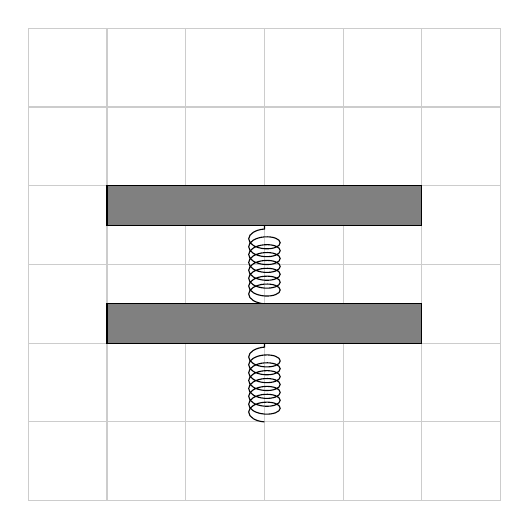
\begin{tikzpicture}
\tikzstyle{rectfill} = [color=black!50,draw=black]
\tikzstyle{mycoil} = [decorate,decoration={coil,segment length=0.1cm,amplitude=0.2cm}]
\draw[step=1.0cm,color=black!20] (-3,-1) grid (3,5);
\draw[mycoil] (0,0) -- (0,1); 
\draw[mycoil] (0,1.5) -- (0,2.5); 
\filldraw[rectfill]  (-2,1.5) rectangle (2,1.0);
\filldraw[rectfill] (-2,2.5) rectangle (2,3.0);
\end{tikzpicture}
\end{center}

\begin{center}
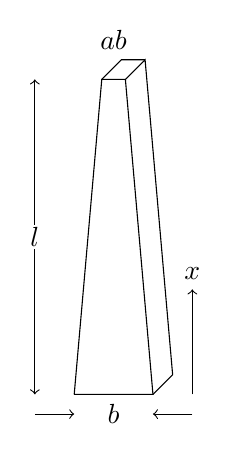
\begin{tikzpicture}
\tikzstyle{ann} = [fill=white,inner sep=1pt]
\def\a{0.3}
\def\b{1}
\def\l{4}
\draw (-\b/2,0)       
   -- (-\b*\a/2,\l)   
   -- (\b*\a/2,\l)    
   -- (\b/2,0)        
   -- (-\b/2,0);
\draw (\b/2,0) -- (\b/2+0.25,0.25) -- (\a*\b/2+0.25,\l+0.25) -- (\a*\b/2,\l);
\draw (\a*\b/2+0.25,\l+0.25) -- (-\a*\b/2+0.25,\l+0.25) -- (-\a*\b/2,\l);
\draw[<->] (-\b,0) -- (-\b,\l);
\draw[->]  (-\b,-0.25) -- (-\b/2,-0.25);
\draw[->]  (\b,-0.25) -- (\b/2,-0.25);
\draw[->]  (\b,0) -- (\b,\l/3) node[anchor=south] {$x$};
\node[ann] at (-\b,\l/2) {$l$};
\node[ann] at (0,-0.25) {$b$};
\node[ann] at (0,\l+0.5) {$ab$};
\end{tikzpicture}
\end{center} 



\begin{center}
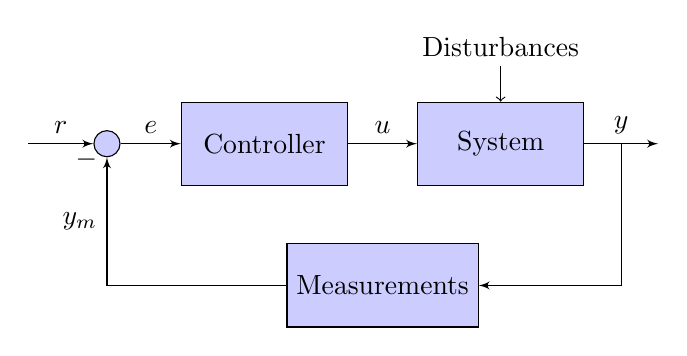
\begin{tikzpicture}[auto, node distance=2cm,>=latex']
\tikzstyle{block} = [draw, fill=blue!20, rectangle, 
    minimum height=3em, minimum width=6em]
\tikzstyle{sum} = [draw, fill=blue!20, circle, node distance=1cm]
\tikzstyle{input} = [coordinate]
\tikzstyle{output} = [coordinate]
\tikzstyle{pinstyle} = [pin edge={to-,thin,black}]
    % We start by placing the blocks
    \node [input, name=input] {};
    \node [sum, right of=input] (sum) {};
    \node [block, right of=sum] (controller) {Controller};
    \node [block, right of=controller, pin={[pinstyle]above:Disturbances},
            node distance=3cm] (system) {System};
    % We draw an edge between the controller and system block to 
    % calculate the coordinate u. We need it to place the measurement block. 
    \draw [->] (controller) -- node[name=u] {$u$} (system);
    \node [output, right of=system] (output) {};
    \node [block, below of=u] (measurements) {Measurements};

    % Once the nodes are placed, connecting them is easy. 
    \draw [draw,->] (input) -- node {$r$} (sum);
    \draw [->] (sum) -- node {$e$} (controller);
    \draw [->] (system) -- node [name=y] {$y$}(output);
    \draw [->] (y) |- (measurements);
    \draw [->] (measurements) -| node[pos=0.99] {$-$} 
        node [near end] {$y_m$} (sum);
\end{tikzpicture}
\end{center}

\end{document}
